
\section{Experimental Studies}

\begin{itemize}
\item Method tested using the CMA-ES on a few test functions.
\item Illustrative example for different training size and
  kernel types for Rosenbrock's function:
\end{itemize}

\begin{center}
\begin{tabular}{c@{ }c@{ }c}
\resizebox*{0.33\columnwidth}{!}{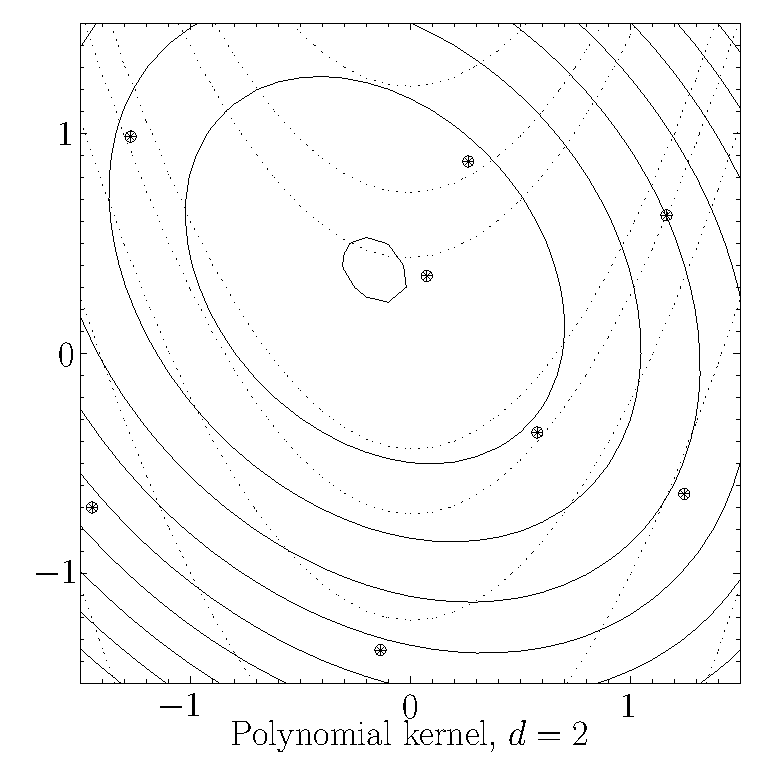
\includegraphics[height=0.33\columnwidth]{figs/poly2global10.eps}} &
\resizebox*{0.305\columnwidth}{!}{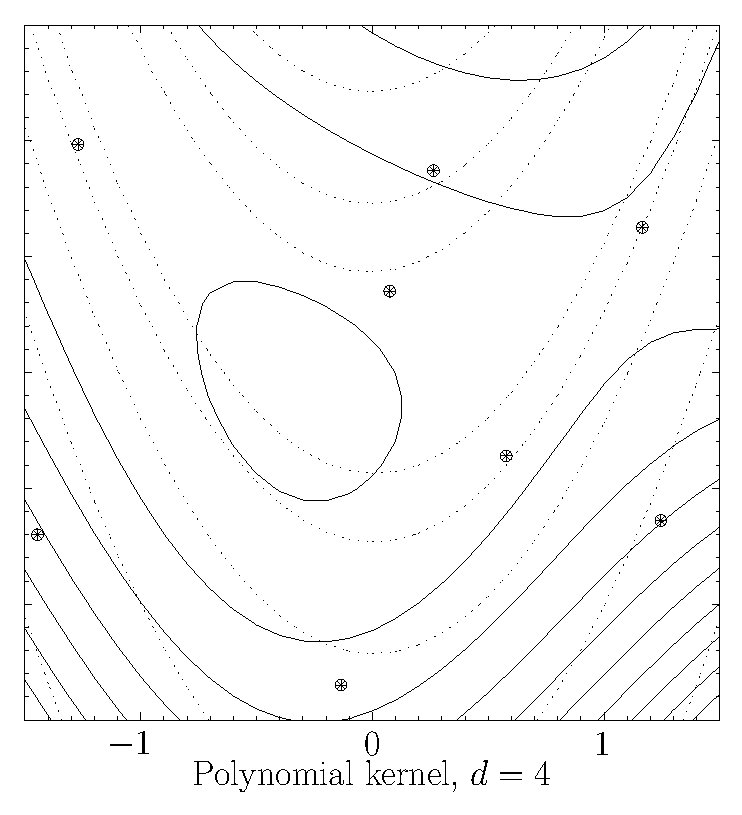
\includegraphics[height=0.33\columnwidth]{figs/poly4global10.eps}} &
\resizebox*{0.305\columnwidth}{!}{\includegraphics[height=0.33\columnwidth]{figs/rbf1global10.eps}} \\
\resizebox*{0.33\columnwidth}{!}{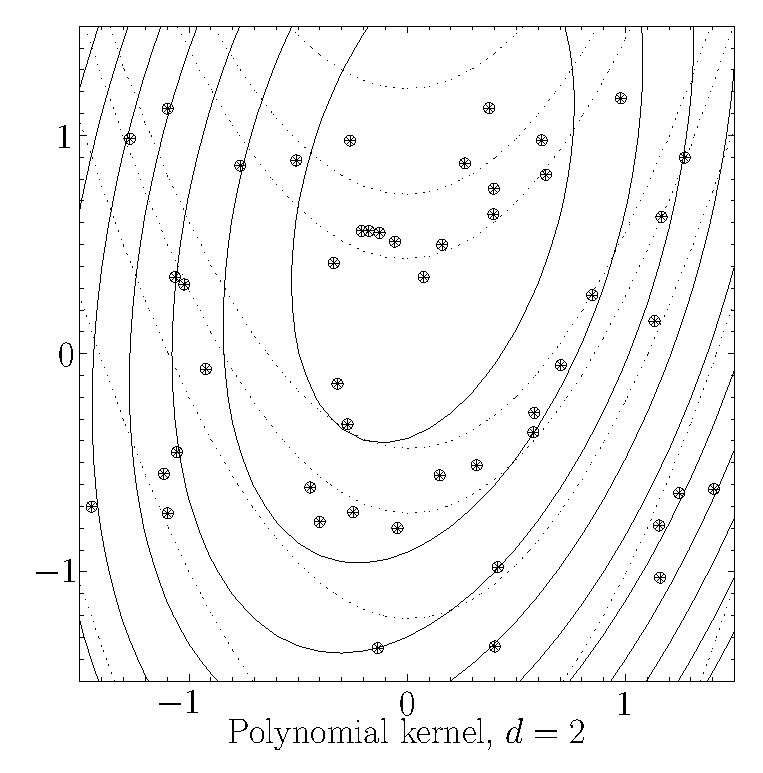
\includegraphics[height=0.33\columnwidth]{figs/poly2global.eps}} &
\resizebox*{0.305\columnwidth}{!}{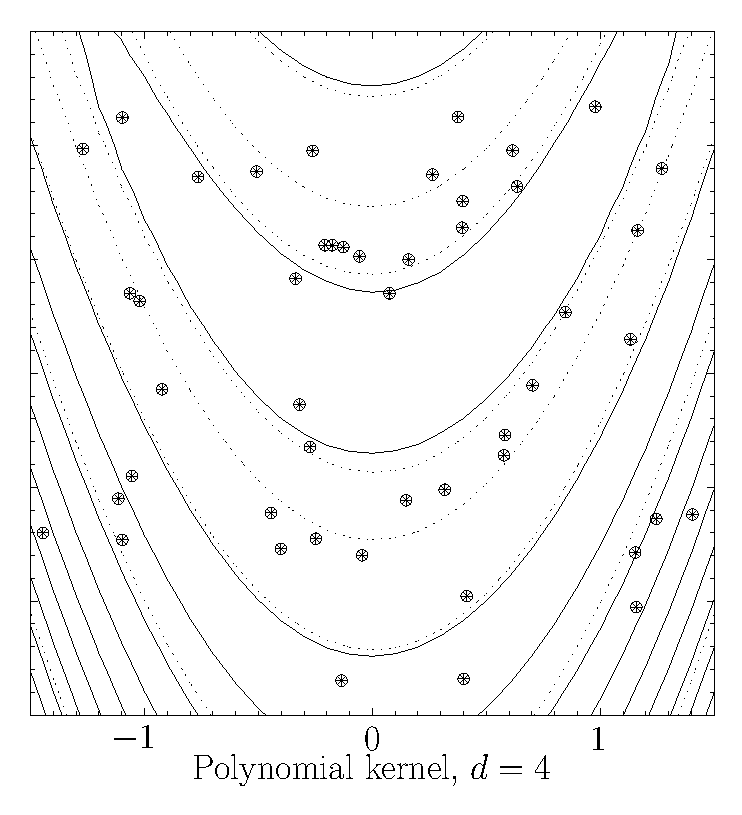
\includegraphics[height=0.33\columnwidth]{figs/poly4global.eps}} &
\resizebox*{0.305\columnwidth}{!}{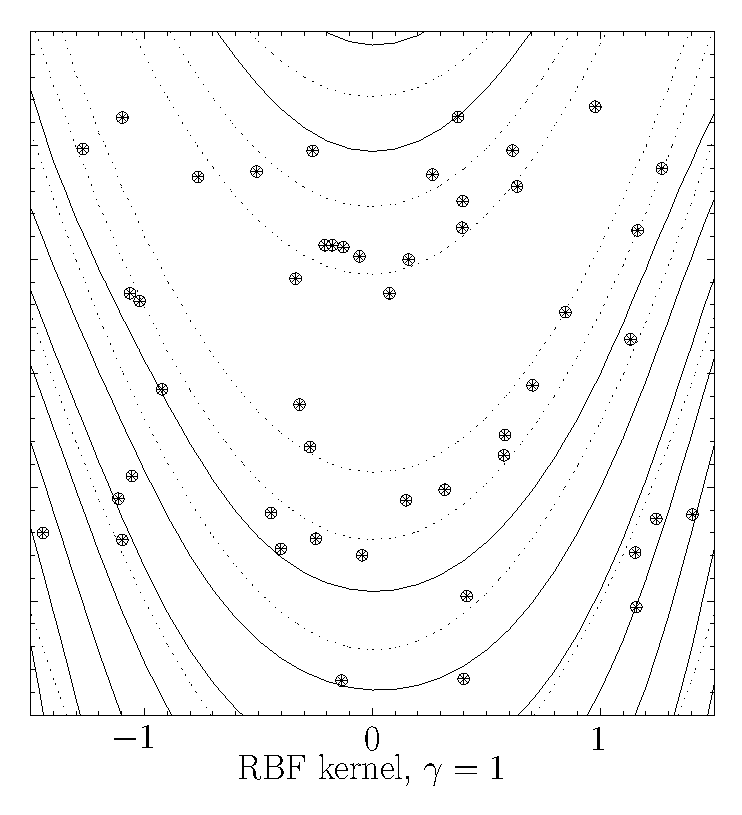
\includegraphics[height=0.33\columnwidth]{figs/rbf1global.eps}} \\
\end{tabular}
\end{center}
